\documentclass{article}[11pt]
\usepackage{Geoff,graphicx}

\title{Different distance functions for Graph Weights\\Some quick notes}
\author{Geoffrey Iyer}

\begin{document}
\maketitle

\section{Statement}

Some quick notation. Working with $n$ points in $\R^n$, let's label the points $x_1,\ldots,x_n$. We're interested in distances between points in different norms. So let
\[D^1 = \left\{\norm{x_i - x_j}_1 \,:\, 1\leq i < j \leq n\right\}\]
\[D^\infty = \left\{\norm{x_i - x_j}_\infty \,:\, 1\leq i < j \leq n\right\}\]
In other words, for each norm there are $n \choose 2$ values that we're interested in. A little bit more notation. Have
\[d_{ij}^1 = \norm{x_i - x_j}_1\]
\[d_{ij}^\infty = \norm{x_i - x_j}_\infty\]
\begin{theorem} Given arbitrary orderings on the sets $D^1,D^\infty$, it's possible to choose the $x_1,\ldots,x_n$ such that the normal ordering with respect to $<$ on each set agrees with the ordering chosen.

  In other words, by picking the $x_1,\ldots,x_n$, we can simultaneously order the distances in both norms however we want.
\end{theorem}

\begin{cor} A similar result can be proven for any two choices of norms, $L^p$ and $L^q$.
\end{cor}
\begin{proof}
  It's pretty easy to adapt the result with $L^1$ and $L^\infty$. The same thing can be done, with just a little more care.

  Actually, it might even be completely free. Isn't it the case that the function $p \mapsto \norm{x}_p$ is monotone decreasing? I'll look over this more carefully later.
\end{proof}

\section{Heuristics}

The idea behind this theorem is that it's always possible for a change in norm to radically change the optimal graph cut. For example, suppose we are working with a dataset that has 3 main clusters, and we're trying to segment it into 2 pieces. Roughly speaking, each cluster can be represented by one point (one of the $x_i$ above). Then even in a dimension as small as $R^2$ or $R^3$, it's possible for a change in norm to change the ordering of the distances in such a way that a whole cluster is classified differently.

\section{Possible extensions}

If you look at the proof carefully you'll notice that the difference between the different distances in the examples created is very small. Enough is done to create the ordering desired, but in reality a lot of the different distances are practically equal. Therefore, if one were to actually use these examples and look at the different graph cuts, I don't think a lot would actually change. So if we were to continue to pursue this topic I think this would be the next interesting area.

It boils down to the tightness of the bound we get from equivalence of norms. We have that
\[dist_\infty(x_i,x_j) \leq dist_1(x_i,x_j) \leq n\cdot dist_\infty(x_i,x_j),\]
but how much do the values vary within this bound? In the example created below, each distance $d_{ij}^1$ is roughly 2 times $d_{\ell k}^\infty$. So in this case the above bound is very loose.

In total, I think some result can be obtained that's along the lines of: ``Given a change of norm, the number of points that change class in the optimal graph cut is bounded by something or another''.

\section{Proof}
\begin{proof}
  Not a full formal proof, but at least the main ideas. Begin with just the standard basis vectors
  \[x_i = e_i \quad 1\leq i \leq n\]
  Here, $d_{ij}^1 = 2, d_{ij}^\infty = 1$ for all $i,j$. We then proceed to make small edits to the $x_i$ to achieve the desired order. By ``edits'', I mean one of two specific moves. We can adjust $d_{ij}^1$ by editing $x_i$ via
  \begin{align}\label{eqn:move1}
    x_i^{new} = x_i^{old} + \epsilon\cdot e_j\quad\text{for some }\epsilon < 1,
  \end{align}
  as pictured in figure \ref{fig:move1}. This decreases $d_{ij}^1$ by $\epsilon$, increases $d_{i\ell}^1$ by $\epsilon$ for $\ell \neq j$, and does not affect $d_{\ell k}^\infty$ for any $\ell, k$.

  The second ``edit'' is
  \begin{align}\label{eqn:move2}
    x_i^{new} = x_i^{old} + \epsilon\cdot e_j - \epsilon\cdot e_i \quad\text{for some }\epsilon < 1,
  \end{align}
  as pictured in figure \ref{fig:move2}. This decreases $d_{ij}^1$ by $2\cdot\epsilon$, decreases $d_{ij}^\infty$ by $\epsilon$, and does not affect $d_{\ell k}^\infty$ for any $\ell, k$.

  Given these two possible moves, it's relatively simple to achieve the desired ordering of distances by using progressively decreasing values of epsilon. At each step one can choose epsilon sufficiently small so that the changes from the previous steps are not affected. (For example, at each step, epsilon is one half of the previous epsilon).
  
  \begin{figure}
    \centering
    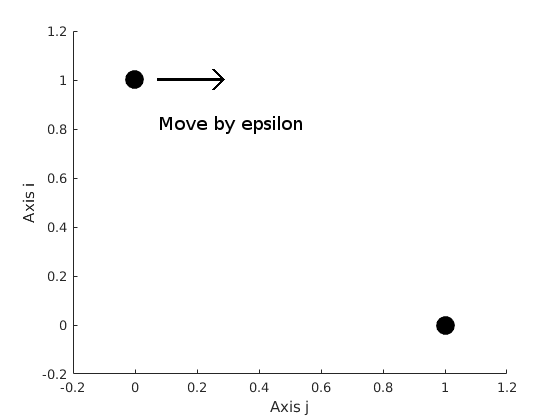
\includegraphics[width = 0.6\linewidth]{move1.png}
    \caption{Move 1}
    \label{fig:move1}
  \end{figure}
  \begin{figure}
    \centering
    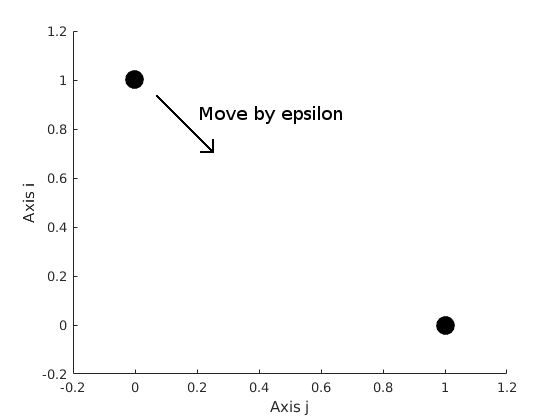
\includegraphics[width = 0.6\linewidth]{move2.png}
    \caption{Move 2}
    \label{fig:move2}
  \end{figure}
\end{proof}

\end{document}
